\documentclass[9pt,twocolumn,twoside]{styles/osajnl}
\usepackage{fancyvrb}
\usepackage[colorinlistoftodos,prependcaption,textsize=normal]{todonotes}
\newcommand{\TODO}[2][]{\todo[color=red!10,inline,#1]{#2}}
\newcommand{\GE}{\TODO{Grammar}}
\newcommand{\SE}{\TODO{Spelling}}
\newcommand{\TE}{\TODO{Term}}
\newcommand{\CE}{\TODO{Citation}}
\journal{i524} 

\title{CDAP Cask Data Application Platform}

\author[1,*, +]{Avadhoot Agasti}

\affil[1]{School of Informatics and Computing, Bloomington, IN 47408, U.S.A.}

\affil[*]{Corresponding authors: aagasti@indiana.edu}

\affil[+]{HID - SL-IO-3000}

\dates{project-000, \today}

\ociscodes{CDAP, Hadoop}

% replace this with your url in github/gitlab
\doi{\url{https://github.com/avadhoot-agasti/sp17-i524/tree/master/paper1/S17-IO-3000/report.pdf}}


\begin{abstract}
This paper explains CDAP - Cask Data Application Platform. CDAP provides
abstraction layer on top of Apache Hadoop and other Apache Big Data Stack
technologies. This paper explains CDAP technology, the kind of problems it
can solve, the infrastructure and setup requirements, and its competitive
landscape. The paper also provides links to learning material for
CDAP.
\newline
\end{abstract}

\setboolean{displaycopyright}{true}

\begin{document}

\maketitle

\TODO{This review document is provided for you to achieve your
  best. We have listed a number of obvious opportunities for
  improvement. When improving it, please keep this copy untouched and
  instead focus on improving report.tex. The review does not include
  all possible improvement suggestions and if you sea comment you may
  want to check if this comment applies elsewhere in the document.}
\TODO{Abstract: remove This paper, its clear that this is a a paper so you do
  not have to mention it. Furthermore, its actually a technology
  review. Abstract has grammar errors.}

\section{Introduction}

CDAP stands for Cask Data Application Platform \CE. CDAP is an
application development platform using which developers can build,
deploy and monitor applications on Apache Hadoop. \TODO{Grammar, make
  sure you check grammar we will not point out every grammer \SE or
  spelling error} In a typical CDAP application, a developer can
ingest data, store and manage datasets on Hadoop, perform batch mode
data analysis, and develop web services to expose the data.  They can
also schedule and monitor the execution of the application. This way,
CDAP enables the developers to use \GE single platform to develop the
end to end \SE application on Apache Hadoop.  This paper introduces
\TODO{not needed phrase this paper, try to avoid, Instead be concreate \SE
  and say the paper is structured as follows. IN Section ... we do,
  use Latex refs and labels} CDAP as application development platform
and explains various use cases that can be solved using CDAP. The
paper also explains the CDAP deployment options and infrastructure
requirements.  Finally we conclude by explaining the other similar
platforms and their high level comparison with CDAP.  The paper also
provides references to the learning material \GE.

\section{Why CDAP}
\TODO{Do not use questions in section headers, and if, you need a ?} 
Before we understand how CDAP helps in application development, lets understand
how a typical application looks like in Hadoop.
\TODO{not a good way to introduce this section}

\subsection{Typical Application Architecture on Hadoop}
Figure 1 \TODO{not using refs and labes for images} shows a typical application architecture on Hadoop.
\TODO{now what, are you explaining it?}

\begin{figure}[htbp]
\centering
\fbox{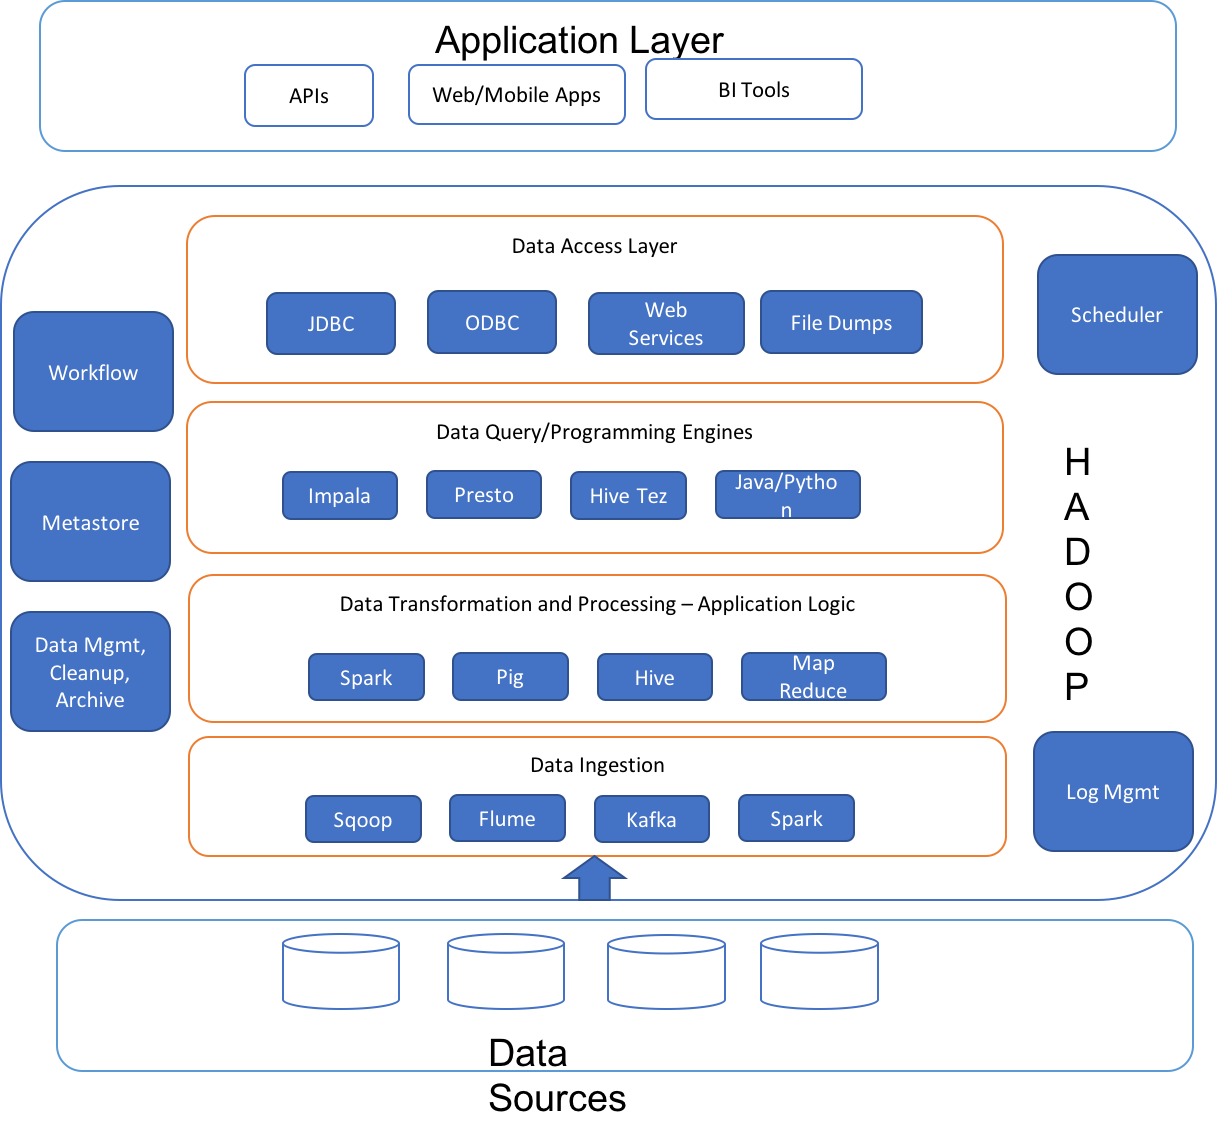
\includegraphics[width=\linewidth]{images/hadoop-application-arch.png}}
\caption{Typical Application Architecture on Hadoop. \TODO{Is this
    copied, if so you need refernce\TODO{You have not used spell checker}. If self drawn, change image to
    not use white fonts on dark background but use black fonts, make
    contrast high e.g. boxes lighter so we can read, make sure
    fontsize is ok and readable} \TODO{where is CDAP in this figure?}}
\label{fig:hadoop-arch}
\end{figure}

There are following layers/components - \GE \TODO{in english you use :}

\TODO{use latex description}
\TODO{inconsistent capitalization}
\begin{itemize}
\item Data Ingestion - ingest the data from data source into Hadoop.
Data Ingestion tools like Apache Sqoop \CE, Apache Flume \CE, Apache
Kafka \CE are
popularly used \TE for Data Ingestion
\item Data Storage - The data is stored in HDFS \CE.
\item Data Processing - The data is transformed and aggregated in Data
Processing layer. The processing can involved \GE various steps like cleansing,
joining, aggregation and running machine learning algorithms. Many different
tools and technologies are used to perform data processing operations
- e.g. \TODO{avoid e.g. here you may want to use such as}
PIG, Hive, Spark are popular open source scripting technologies while
Talend, Informatica are visual commercial products.
\item Result Storage - The output of data processing step \GE is again stored in
HDFS \TODO{why again?}
\item Data Access - The end users can \TODO{is can needed?} access the data (mainly results)
using various data access mechanism like APIs, SQL interface or BI tool
interface. \TODO{do you need a/an/the?}
\end{itemize}

\subsection{Why CDAP - CDAP Application Architecture}
\TODO{avoid question in section header}
CDAP provides a common application development platform in which a developer
can code all the application layers in a typical Hadoop application. 
\TODO{Is this repetition or something new. If it is something new,
  than say in addition to xyz CDAP provides ....}
CDAP
provides abstractions to ingest data, store it in HDFS, process it using
the application business logic, store the results in HDFS and expose web
service APIs on the result data. 
\TODO{It is unclear if this is new or already explained, see the list
  you had previously}
User \GE need not use different tools to code
different layers. He can simply code all the layers in CDAP platform. He can
use \GE same coding language (Java) to do the coding across all the layers.

Further \TE CDAP uses native Hadoop tools for actually performing the operations.
 For example, the data processing operation implemented in CDAP translate to
 Spark jobs \CE. Due to this, CDAP users continue to leverage the new
 enhancements in Apache Hadoop.\TODO{Which new enhancements?}\CE


\section{Important CDAP Concepts}
CDAP revolves around \TE below important concepts:
\begin{itemize}
\item CDAP Datasets provide logical abstraction \GE over the data stored in
Hadoop. The data can be files in HDFS or tables in HBase. A dataset needs to
be first declared in the CDAP. Any dataset declared in CDAP can be used in
any CDAP applications or CDAP services.
\item CDAP Applications provide containers to implement application business
logic in open source processing frameworks like map reduce, Spark and real
time flow. CDAP applications also provide standardize way to deploy and
manage the apps
\item CDAP Services provide services for application management, metadata
management, and streams management
\end{itemize}
\TODO{this seems in part replication of what was said before, would it
  be worth while to combine sections. Also should concepts not before architecture?}


\section{CDAP Deployment}
CDAP provides many deployment options. In standalone mode, it can be
downloaded as a zip file and deployed.
Alternatively it is available as a standalone virtual machine.
For cluster mode deployment, CDAP provides \GE Hadoop-distribution specific
options as explained below
\begin{itemize}
\item Cloudera Hadoop Distribution (CDH) \CE- Cloudera Manager \CE is tool to
 deploy CDH cluster. As per CDAP documentation \TODO{not helpful to
   say its in the documentation without listing the reference}
\cite{www-cdap-cloudera-manager} CDAP provides CDAP-parcel \CE which
is \GE plug in for
Cloudera Manager. Once you add CDAP-parcel
to your Cloudera Manager, CDAP can be deployed using Cloudera Manager and all
 CDAP services can be monitored using Cloudera Manager \TODO{full stop}
\item Amazon EMR (Elastic Map Reduce) - EMR \CE is Amazon's Hadoop distribution
for the Amazon Web Services cloud. EMR provides \GE 'Create Cluster Wizard' to
create EMR cluster. According the CDAP documentation \cite{www-cdap-emr}, CDAP
provides a bootstrap action which is executed when the EMR cluster is created
. Using this mechanism, \GE CDAP platform can be deployed on EMR when the EMR
cluster is created.
\end{itemize}
\TODO{inconsistent use of list as horton is outside of list}
CDAP can also be deployed on HortonWorks Hadoop Distribution, MapR Hadoop
Distribution and Apache Hadoop.



\section{CDAP Infrastructure Requirements}

CDAP is deployed on edge nodes \TODO{what is an edge node} of the Hadoop cluster. CDAP communicates with
Hadoop services like Yarn\CE, HDFS \CE and HBase \CE. Hence CDAP needs to be installed
in \GE same network as that of Hadoop. However, none of the CDAP components are
required to be installed on Hadoop Namenode \TODO{what is a name node}\CE
or Hadoop datanodes. CDAP
documentation \cite{www-cdap-deployment} provide \GE the CDAP deployment
architecture.

\section{Educational Material}

\TODO{Paper writing rules do not allow a section to just have a list,
  it must have an introductory sentence}

\begin{itemize}
\item CDPA Applications code repository in Github \cite{github-cdap-apps}
provide sample applications which are built on top of CDAP Platform.
\item CDAP Documentation \cite{www-cdap-getting-started} provides introduction
 to CDAP platform.
\end{itemize}

\TODO{You make a big deal in the abstract but you have only two links, thats
fine, but people wonder why you emphasize this that much}

\section{Representative Use Cases which can leverage CDAP}

\TODO{Introductory sentence missing}
\TODO{inconsistent enumeration, between CASK and Customer 360, while
  using introduction section just for CASK and not Customer 360}

CASK \cite{www-cask-io} is the company which provides commercial distribution
for CDAP. CASK has developed several applications using CDAP.
Some of the applications developed using CDAP are explained below
\begin{itemize}
\item CASK Hydrator \cite{www-cask-hydrator} is interactive application for
building, running and managing data pipelines for enterprise data lake.
CASK Hydrator is UI driven tool using which users can ingest data from
sources like traditional RDBMS, trasnform \TODO{You have not used
  spell checker} it,
aggregate it and finally store the data into permanent storage like HDFS.
CASK Hydrator provides UI drag-and-drop style abstraction to all of the above
 task.
\item Customer 360 is another representative application which can be built
using CDAP. Customer 360 applications analyzes
customer behavior data on various interaction platforms like mobile apps,
online communities, customer support portals,
and social media. CDAP can be used to ingest the data from these sources and
perform join, unification and aggregations to derive 360 degree view of
customer.
\end{itemize}

\section{Licensing}
CDAP is licensed \cite{www-cdap-license}under Apache License,
Version2.0.
\TODO{mind spaces after citations}

\section{Other Hadoop Application Development Platforms}

\TODO{Introductory sentence missing}

\begin{itemize}
\item Cascading \cite{www-cascading} is another application development
platform on Apache Hadoop. Cascading has many similar features like CDAP.
Cascading supports Java APIs, Data Processing APIs, Data Integration APIs,
Scheduler APIs, Relational Operations and scriptable interface. Cascading
also support many different Hadoop distributions.

\item Talend Big Data Integration \cite{www-talend} : Talend is integration
tool using which data can be extracted from source systems, stored on Hadoop
and processed in Hadoop. Although Talend is not exactly an application
development platform, lot of its features overlap with CDAP. Talend provides
visual interface for performing data ingestion and processing operations on
Hadoop
\end{itemize}

\TODO{vage comparison is used, lots of ... can you be more specific}

\section{Conclusion}
CDAP provides an application development platform over Apache Hadoop. Using
CDAP developers can code multiple layers of thier \TODO{You have not
  used spell checker} data pipeline in one
uniform language and tool. \TODO{I do not understand} CDAP also can help to shield developers from
different Hadoop deployment options like Cloudera, Hortonworks and
EMR. \TODO{Not clear enough phrased}

\section*{Acknowledgements}

The authors thank Prof. Gregor von Laszewski for his technical guidance.

\TODO{many citations missing}

% Bibliography

\bibliography{references}

\listoftodos

\end{document}
